%*****************************************
% Lab 02: Adder
%*****************************************
\chapter{Adder}\label{add}

\section{Purpose}

This lab builds a full 1-bit adder, but the intent is to continue to familiarize students with \LE and how basic arithmetic functions can be completed using simple gate-level logic. Additionally, this lab develops an automated testing system that will be used to test future lab submissions.

\section{Procedure}

\subsection{Half-Adder}

Open Logisim and start a new project. In \LE circuits can contain any number of sub-circuits. Subcircuits fill the same role in a physical circuit as a function or procedure fills in a software project. A new subcircuit can be added to a circuit by clicking \textsc{Project -> Add Circuit}. Name the new circuit \lstinline[columns=fixed]|Half_Adder|. Open the new subcircuit by double-clicking its name in the Explorer Pane. 

Because this is a new subcircuit, the drawing canvas is blank. A half-adder is a circuit that will add two input bits. Because it is possible to add two bits and generate a carry, the half-adder must allow for a carry out bit. Figure \ref{fig:add-01} is the circuit diagram for a half-adder.

\begin{figure}[H]
	\centering
	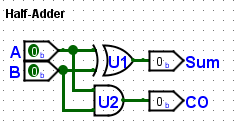
\includegraphics[width=\maxwidth{.95\linewidth}]{gfx/add-01}
	\caption{Half-Adder}
	\label{fig:add-01}
\end{figure}

This is fairly easy to build. Component \texttt{U1} is an \texttt{XOR} gate and \texttt{U2} is an \texttt{AND} gate. There are two inputs and two outputs and all of the devices should be connected as shown. To test the circuit, whenever input \textit{A} and input \textit{B} are different the \textit{Sum} should be high and when input \textit{A} and input \textit{B} are both high the \textit{CO} (Carry Out) bit should also be high.

\subsection{Full Adder}

A full adder takes two input bits and adds them, like a half-adder, but it also includes the logic necessary to input or output a carry bit so it can be cascaded with other adders. Figure \ref{fig:add-02} is the logic diagram for a full adder.

\begin{figure}[H]
	\centering
	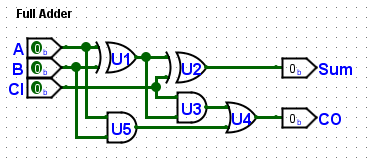
\includegraphics[width=\maxwidth{.95\linewidth}]{gfx/add-02}
	\caption{Full Adder}
	\label{fig:add-02}
\end{figure}

Create a new subcircuit named \lstinline[columns=fixed]|Full_Adder| and wire all of the components as illustrated in Figure \ref{fig:add-02}. Notice that \texttt{U1} and \texttt{U2} are \texttt{XOR} gates, \texttt{U3} and \texttt{U5} are \texttt{AND} gates, and \texttt{U4} is an \texttt{OR} gate. There are also three inputs and two outputs.

\subsection{Main Circuit}

In most \LE projects, the \lstinline[columns=fixed]|main| circuit is used to provide a nice user interface for the project. Typically, various subcircuits are dropped onto the main circuit canvas and various inputs and outputs are wired to them. A user can then test the project without worrying about the details of the subcircuits.

For this project, open the \lstinline[columns=fixed]|main| circuit by double-clicking its name in the Library panel. Click one time on the \lstinline[columns=fixed]|Full_Adder| subcircuit then move the mouse over the drawing canvas. Notice that the mouse pointer has changed into a representation of the subcircuit. Drop that subcircuit anywhere on the drawing canvas and then wire the various inputs and outputs as shown in Figure \ref{fig:add-03}.

\begin{figure}[H]
	\centering
	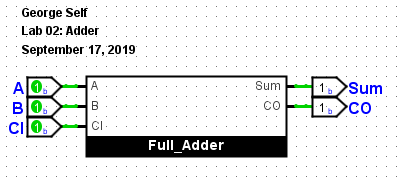
\includegraphics[width=\maxwidth{.95\linewidth}]{gfx/add-03}
	\caption{Full Adder}
	\label{fig:add-03}
\end{figure}

This circuit can be tested by using the \textit{poke} tool and entering these values. After each line, check to see that the outputs are correct.

\begin{table}[H]
	\sffamily
	\newcommand{\head}[1]{\textcolor{white}{\textbf{#1}}}		
	\begin{center}
		\rowcolors{2}{gray!10}{white} % Color every other line a light gray
		\begin{tabular}{ccccc} 
			\rowcolor{black!75}
			\multicolumn{3}{c}{\head{Inputs}} & \multicolumn{2}{c}{\head{Outputs}} \\
			A & B & CI & Sum & CO \\
			\hline
			0 & 0 & 0 & 0 & 0 \\
			0 & 1 & 0 & 1 & 0 \\
			1 & 0 & 0 & 1 & 0 \\
			1 & 1 & 0 & 0 & 1 \\
			0 & 0 & 1 & 1 & 0 \\
			0 & 1 & 1 & 0 & 1 \\
			1 & 0 & 1 & 0 & 1 \\
			1 & 1 & 1 & 1 & 1 \\
		\end{tabular}
	\end{center}
	\caption{Test Vector For Full Adder}
	\label{tab:intro-01}
\end{table}

\subsection{Automated Testing}

While it is possible to use the \textit{poke} tool and check the outputs for various input combinations, as digital logic circuits become more complex it is important to automate the testing process so no input combinations are overlooked. \LE includes a \textsc{Simulate -> Test Vector} feature that is used for automating circuit testing.

The first step in using automatic testing is to create a \textit{Test Vector} file. This is a simple \textit{.txt} file that can be created in any text processor, like \textit{Notepad}. \marginpar{Do not use a word processor to create the Test Vector since that would add unneeded codes for things like fonts and margins.} The format for a test vector is fairly simple.

\begin{itemize}
	\item Every line is a single test of the circuit, except the first line.
	\item The first line defines the various inputs and outputs being tested.
	\item Any line that starts with a hash mark (\#) is a comment and is ignored.
\end{itemize}

Following is the test vector file used to test the \lstinline[columns=fixed]|main| circuit.

\begin{Verbatim}[frame=lines,
numbers=left,
xleftmargin=10mm,
xrightmargin=10mm]
# Test vector for Adder
CI A B Sum CO
0 0 0 0 0
0 0 1 1 0
0 1 0 1 0
0 1 1 0 1
1 0 0 1 0
1 0 1 0 1
1 1 0 0 1
1 1 1 1 1
\end{Verbatim}

Following is an explanation for the \textit{Test vector for Adder} file.

\begin{description}
	\item[Line 1] This is just the title of the file. Because this line starts with a hash (\#) it is a comment and will be ignored by \LE.
	\item[Line 2] This line lists all of the inputs and outputs in the circuit under test. In this case, there are three inputs, \textit{CI}, \textit{A}, and \textit{B}, along with two outputs, \textit{Sum} and \textit{CO}. \LE is able to determine whether the pin is an input or output from its properties. 
	\item[Line 3] This line contains the first test for the circuit. This line specifies that \LE make \textit{CI}, \textit{A}, and \textit{B} equal to zero and then check to be certain that \textit{Sum} and \textit{CO} are also zero.
	\item[Other Lines] All other lines set the three input bits and specify the expected response in the output bits.
\end{description}

To start a test, click \textsc{Simulate -> Test Vector}. The window illustrated in Figure \ref{fig:add-04} opens. 

\begin{figure}[H]
	\centering
	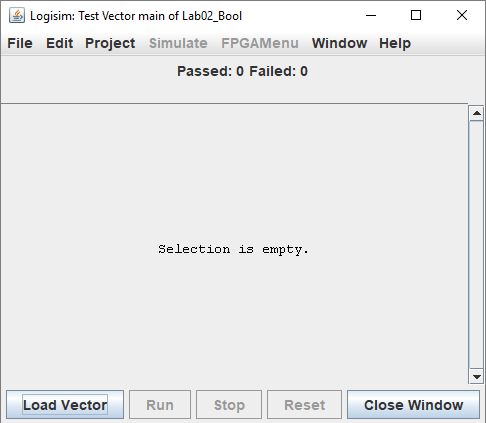
\includegraphics[width=\maxwidth{.95\linewidth}]{gfx/add-04}
	\caption{Test Vector Window}
	\label{fig:add-04}
\end{figure}

Click the \textit{Load Vector} button at the bottom of the window and load the test vector file. The test will automatically start and \LE will report the results, like in Figure \ref{fig:add-05}.

\begin{figure}[H]
	\centering
	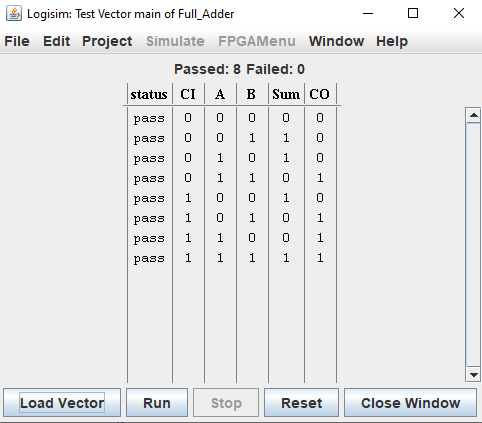
\includegraphics[width=\maxwidth{.95\linewidth}]{gfx/add-05}
	\caption{Test Completed}
	\label{fig:add-05}
\end{figure}

The test indicates all 8 lines passed and zero failed so it could be reasonably concluded that the circuit is functioning properly. Figure \ref{fig:add-06} illustrates a failed test.\marginpar{An error was intentionally added to the test vector file to generate a failed test.} The circuit designer would then need to troubleshoot to determine what went wrong with the circuit.

\begin{figure}[H]
	\centering
	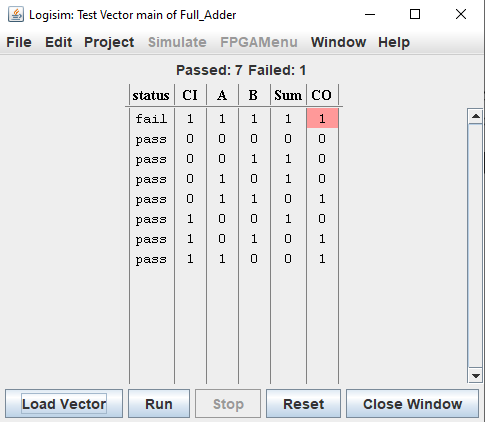
\includegraphics[width=\maxwidth{.95\linewidth}]{gfx/add-06}
	\caption{Test Failure}
	\label{fig:add-06}
\end{figure}

\textit{Note: the test vector files for all labs are made available to students so they can check their work prior to submitting them.}

\section{Deliverable}

To receive a grade for this lab, build both the half-adder and full adder and then add the full adder to the \lstinline[columns=fixed]|main|. It is important to ensure the input and output pin names are the same as in the lab instructions since a test vector will be used to check the circuit. Be sure the standard identifying information is at the top left of the \lstinline[columns=fixed]|main| circuit, similar to: 

\bigskip
% The minipage environment keeps the three lines together - no page break.
\begin{minipage}{\linewidth}
	\begin{verbatim}
	George Self
	Lab 02: Adder
	September 17, 2019
	\end{verbatim}
\end{minipage}
\bigskip

Save the file with this name: \emph{\texttt{Lab02\_Adder}} and submit that file for grading.

